\section{Rob\`otica submarina}

\begin{frame}{Com \`es la meva feina?}
  \keyline{A part de fer classes, treballo amb robots submarins.}
  \begin{columns}[T,onlytextwidth]
    \column{0.49\textwidth}
    \centering
    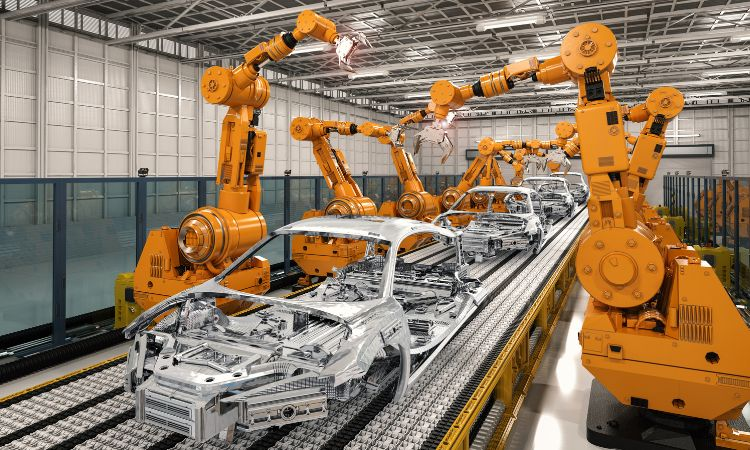
\includegraphics[width=\linewidth,height=0.48\textheight,keepaspectratio]{img/robots-industriales.jpg}
    \\
    {\scriptsize Robot industrial}

    \column{0.49\textwidth}
    \centering
    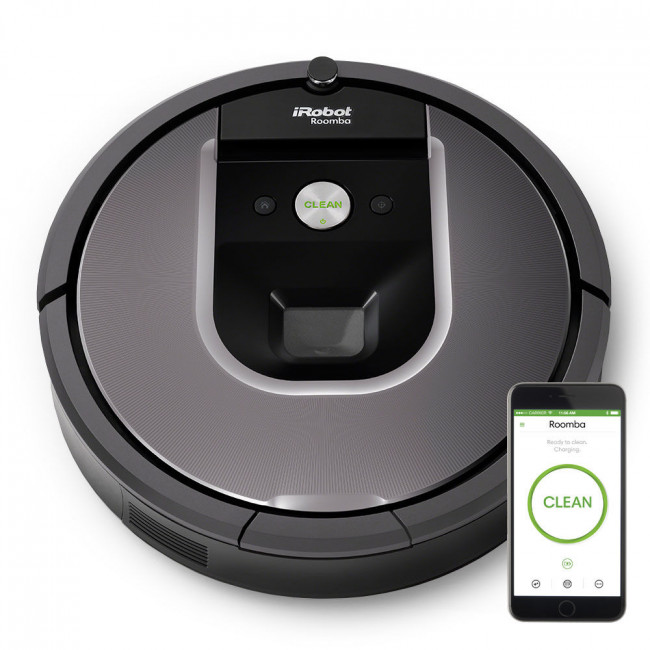
\includegraphics[width=\linewidth,height=0.48\textheight,keepaspectratio]{img/roomba.jpg}
    \\
    {\scriptsize Robot dom\`estic}
  \end{columns}

  \vspace{0.4em}
  \begin{itemize}
    \item La rob\`otica no \`es nom\'es ci\`encia-ficci\'o.
    \item Ens ajuda a fer tasques \`utils a les indústries, a casa i en entorns perillosos com a l'espai o sota l'aigua!
  \end{itemize}
\end{frame}

\begin{frame}{Per qu\`e volem robots sota l'aigua?}
  \keyline{L'oce\`a \`es immens, dif\'icil d'accedir i sovint perill\'os per a persones.}

  \begin{columns}[T,onlytextwidth]
    \column{0.4\textwidth}
    \begin{itemize}
      \item Profunditat, poca llum i mala visibilitat
      \item Dist\`ancies grans i inspeccions llargues
      \item Treballar-hi manualment \`es lent i arriscat
    \end{itemize}

    \column{0.6\textwidth}
    \centering
    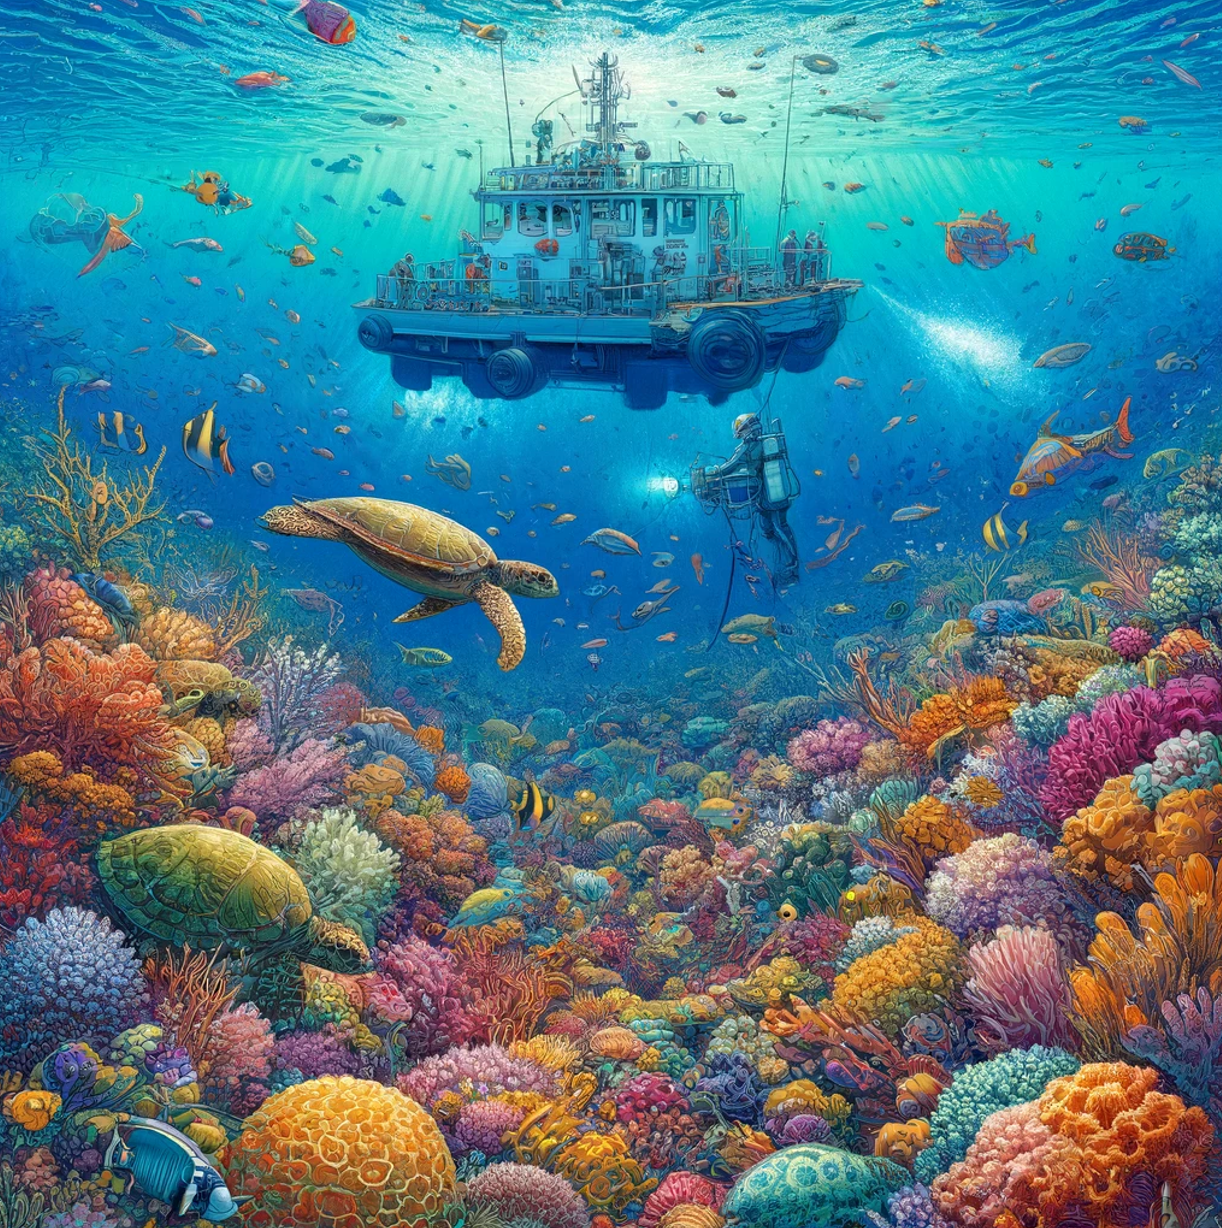
\includegraphics[width=\linewidth,height=0.75\textheight,keepaspectratio]{img/ocean.png}
  \end{columns}

\end{frame}

\begin{frame}{Els "sensits" d'un robot submar\'i?}
  \keyline{Ulls, orelles, cervell i bra\c{c}os per actuar al medi.}

  \begin{columns}[T,onlytextwidth]
    \column{0.45\textwidth}
    \begin{itemize}
      \item \textbf{Ulls}: c\`ameres
      \item \textbf{Orelles}: sonar
      \item \textbf{Cervell}: ordinadors i programari
      \item \textbf{Bra\c{c}os}: manipuladors
    \end{itemize}

    \vspace{0.3em}
    \begin{block}{Entrada $\rightarrow$ proc\'es $\rightarrow$ acci\'o}
      Sensors $\rightarrow$ dades $\rightarrow$ decisions $\rightarrow$ moviment
    \end{block}

    \column{0.55\textwidth}
    \centering
    \fbox{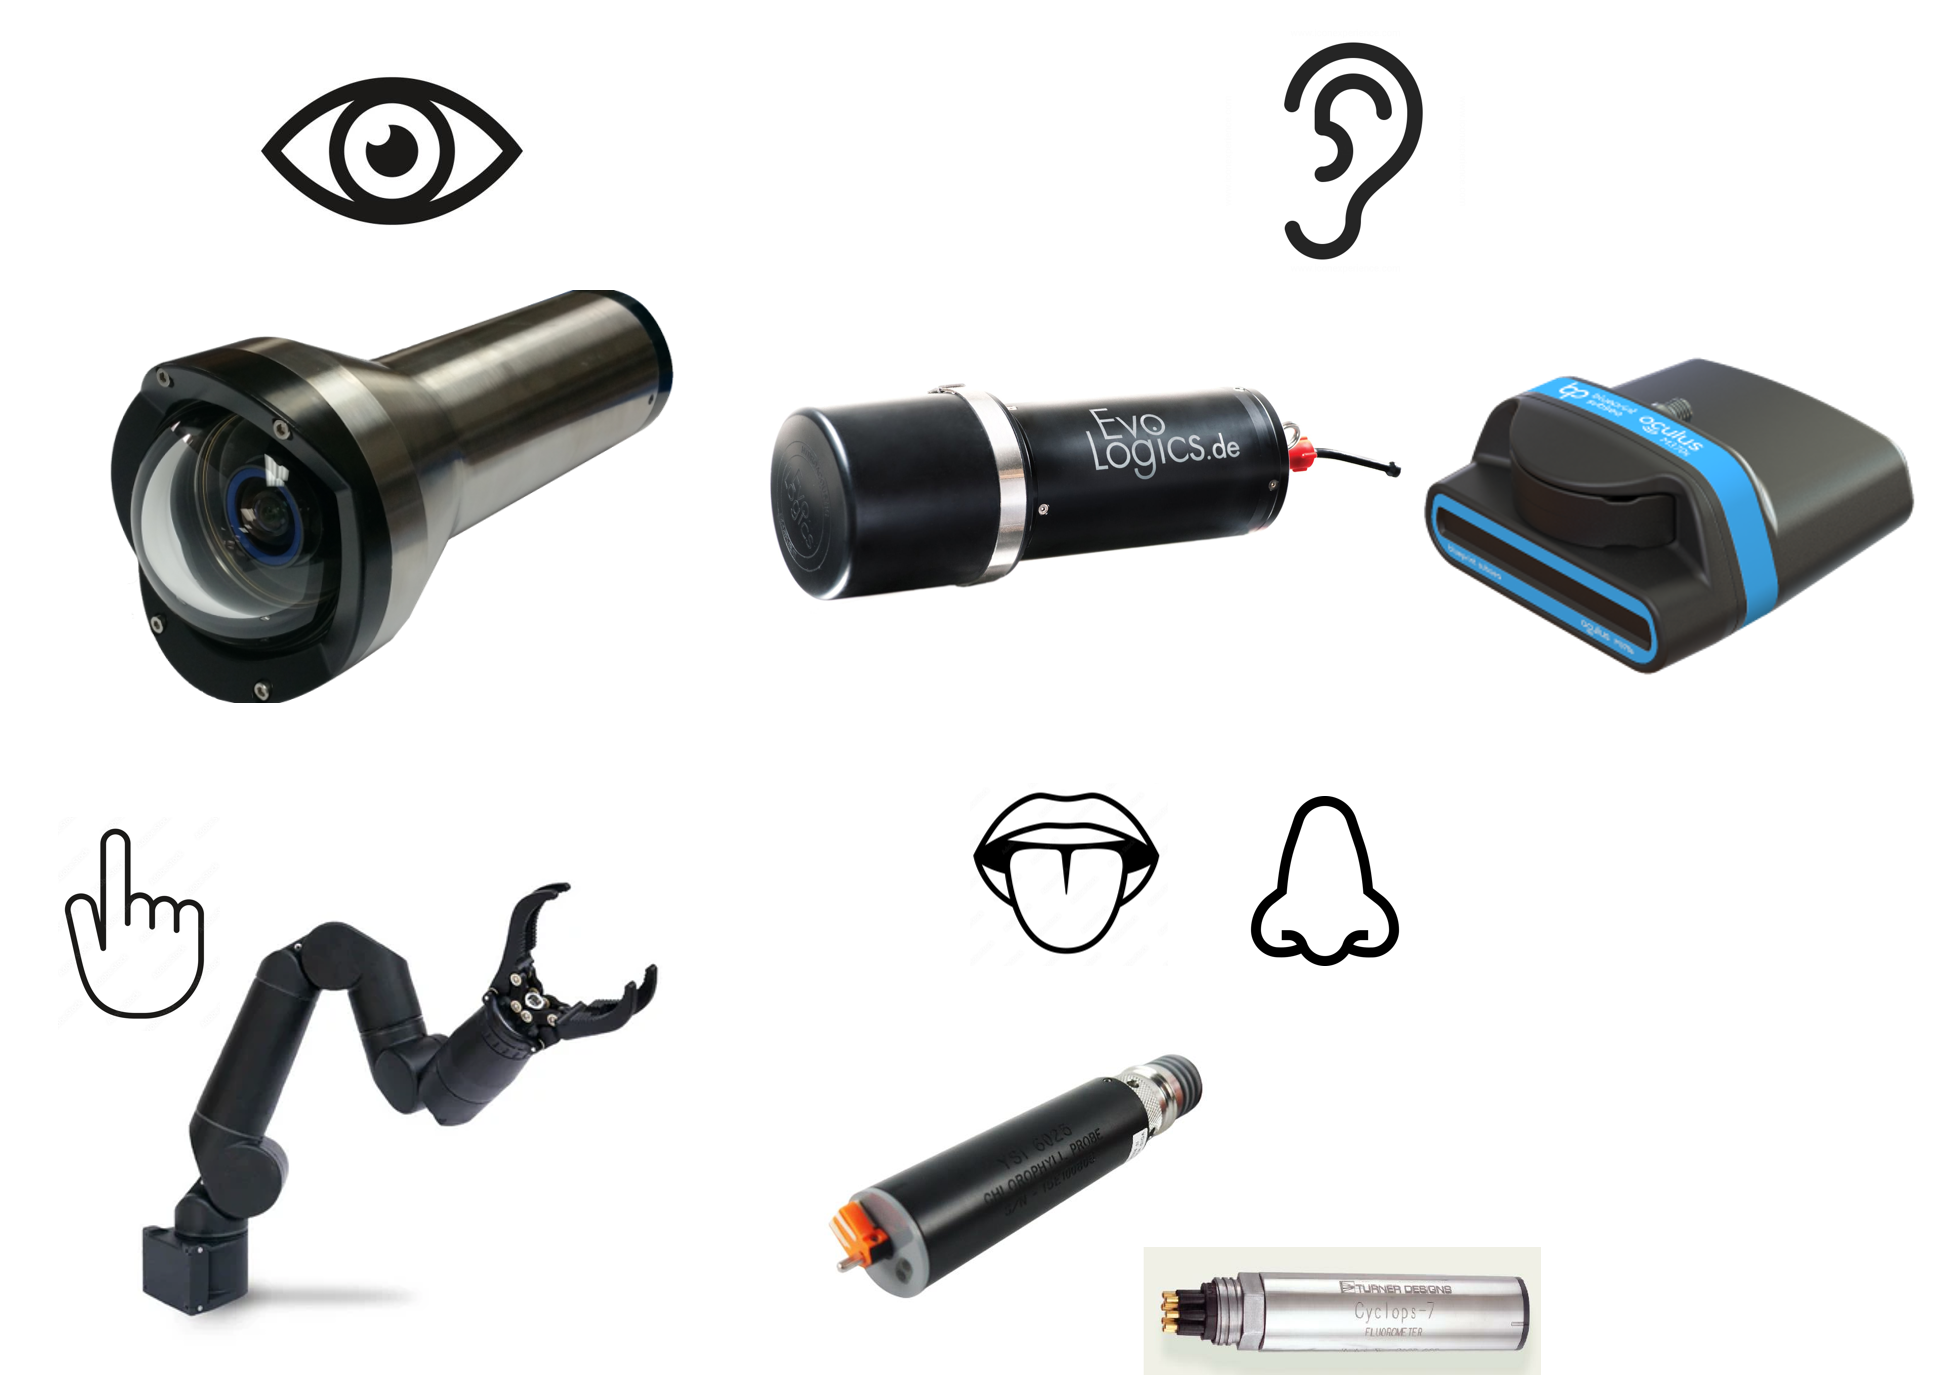
\includegraphics[width=0.9\linewidth]{img/sensors_auvs.png}}
  \end{columns}
\end{frame}

\begin{frame}{Qu\`e podem fer amb aquests robots?}
  \keyline{Ci\`encia, arqueologia, energia i ecologia marina.}

  \centering
  \begin{tabular}{cccc}
    \fbox{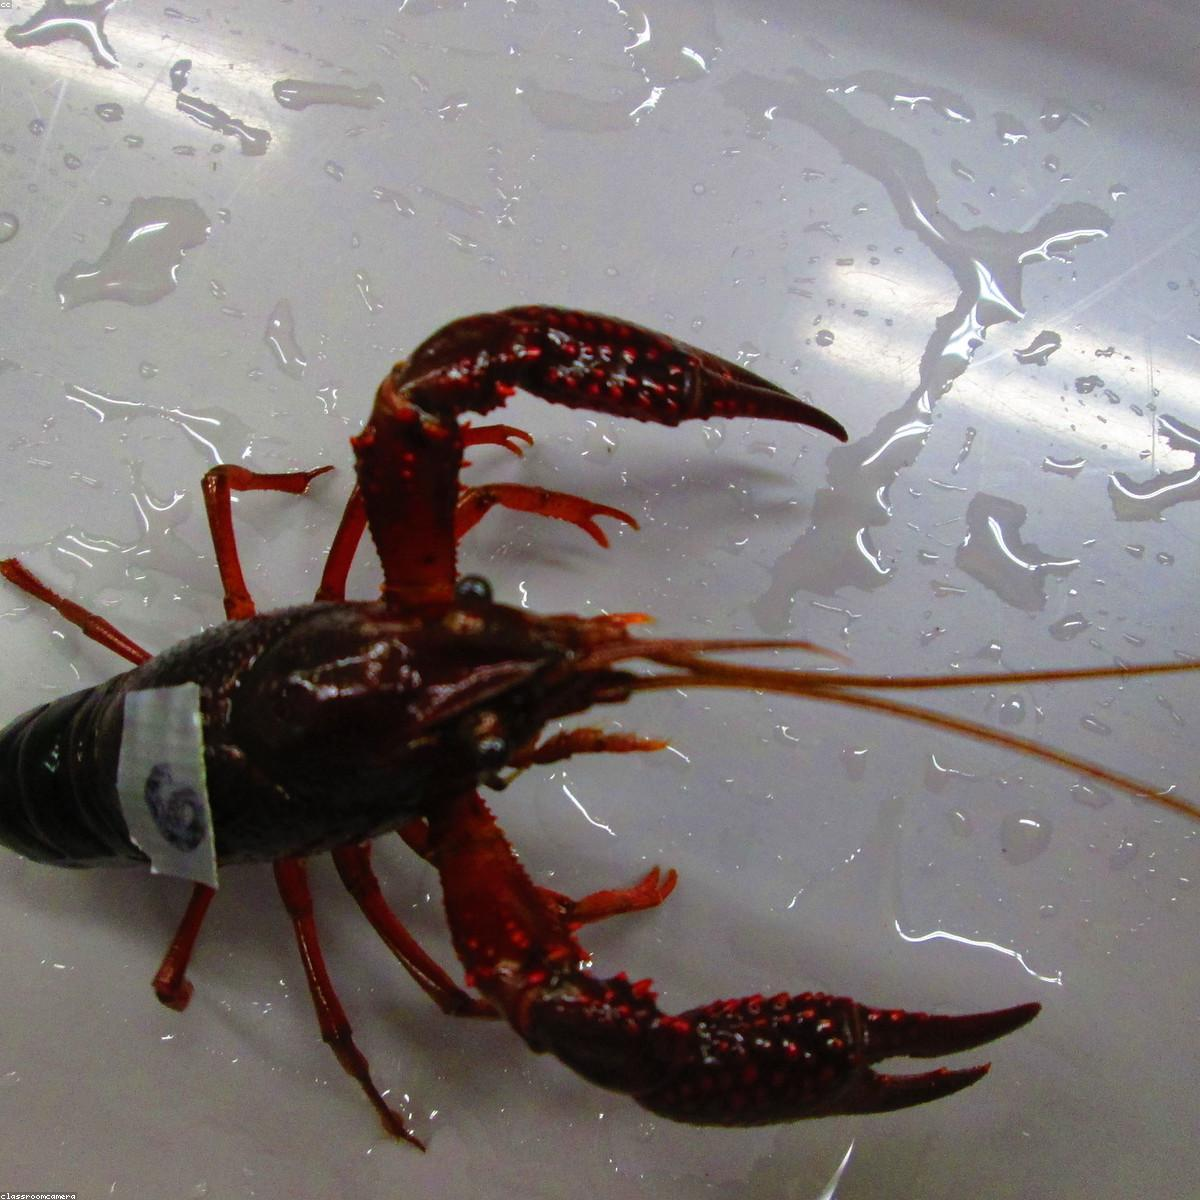
\includegraphics[width=0.2\textwidth]{img/slide29_science.jpg}} &
    \fbox{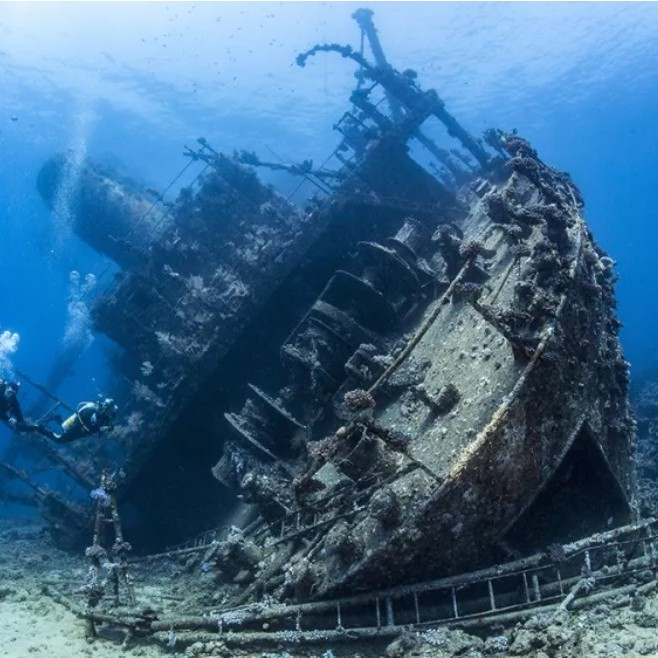
\includegraphics[width=0.2\textwidth]{img/ship_wreck.jpg}}&
    \fbox{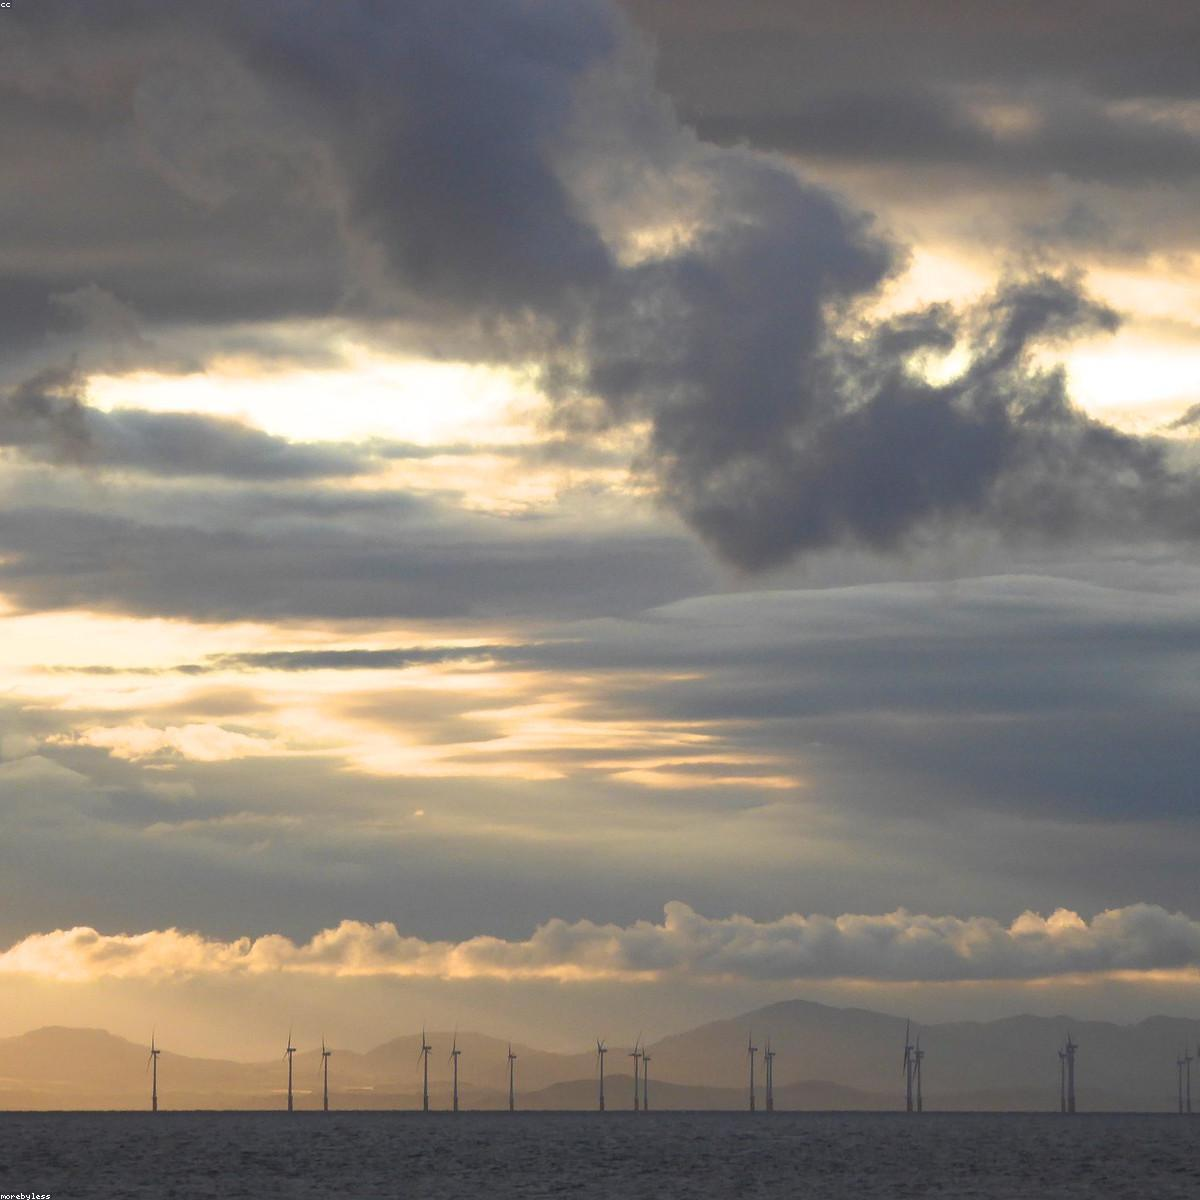
\includegraphics[width=0.2\textwidth]{img/slide29_energy.jpg}} &
    \fbox{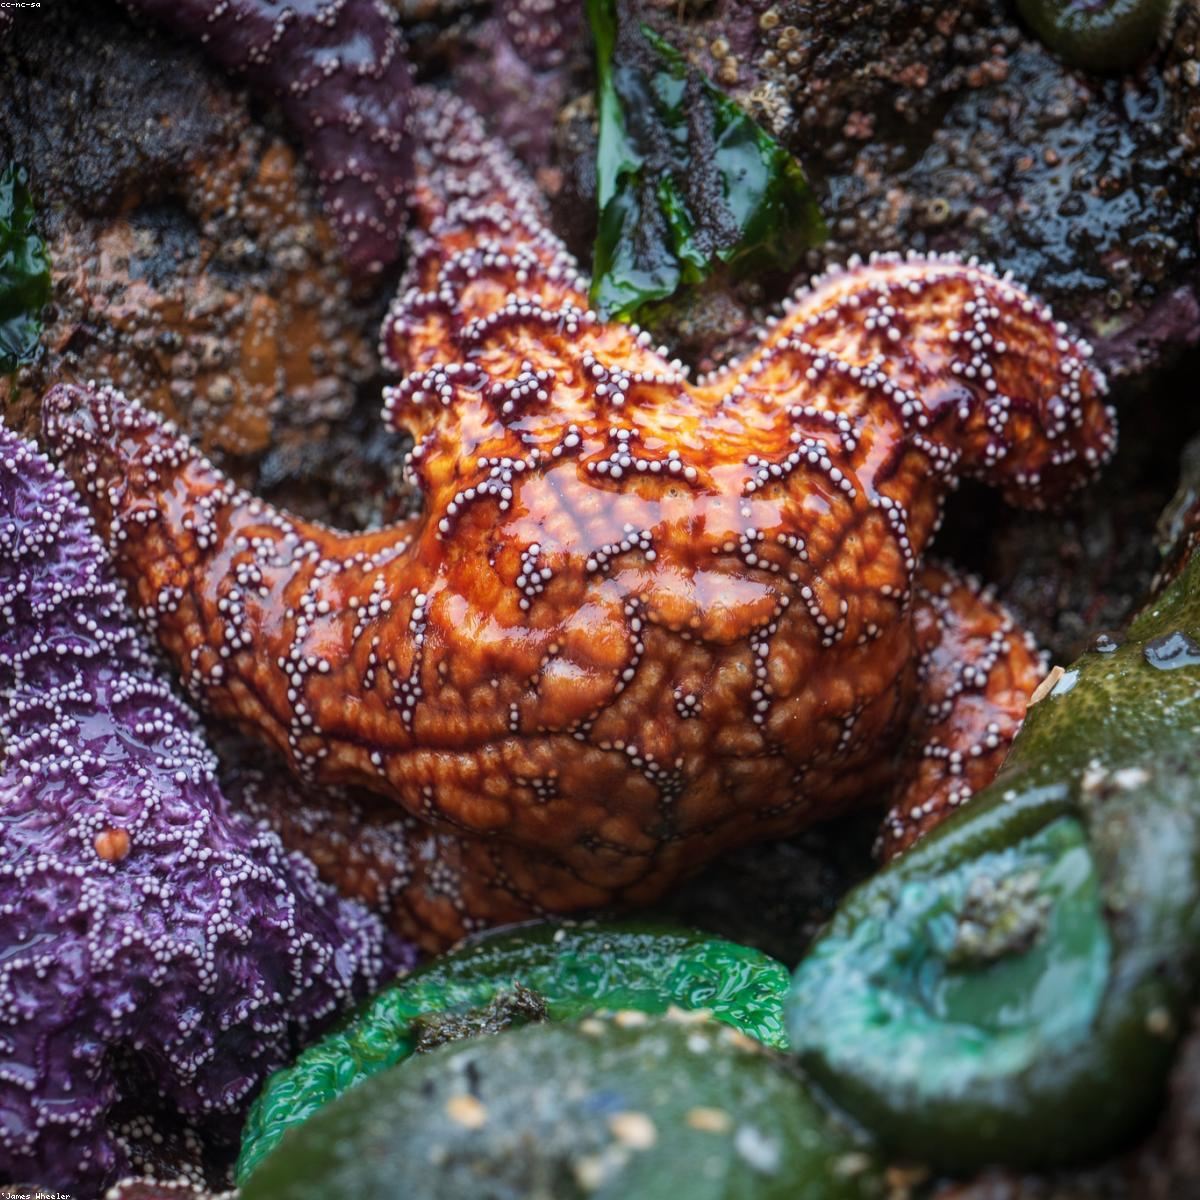
\includegraphics[width=0.2\textwidth]{img/slide29_ecology.jpg}} \\
     \\
    {\scriptsize \textbf{Ci\`encia}} & {\scriptsize \textbf{Arqueologia}} &
    {\scriptsize \textbf{Energia}} & {\scriptsize \textbf{Ecologia}} \\
  \end{tabular}

  \vspace{0.3em}
  {\normalsize La rob\`otica submarina ajuda a con\`eixer i cuidar el mar.}
\end{frame}

\begin{frame}{Algunes coses que hem fet nosaltres}
  \keyline{Projectes i demostracions del canal del CIRS UdG.}

  \begin{itemize}
    \item \href{https://www.youtube.com/watch?v=yE8uoI9v33Q}{Inspection of an Underwater Structure}
    \item \href{https://www.youtube.com/watch?v=4nYtELVcGMA}{Underwater Pose SLAM using GMM Scan Matching for a Mechanical Profiling Sonar}
    \item \href{https://www.youtube.com/watch?v=RfvtNYkLQvM}{Autonomous Cooperative Underwater Object Assembly}
  \end{itemize}

\end{frame}
